A la hora de tener que representar un partido, llegamos a que un partido conoce a dos equipos, los que se van a enfrentar entre si y además hay una noción de que un partido se va desarollando através de turnos, los cuales finalizan cuando la pelota o bien entra al aro de basket o se va de la cancha. Una vez finalizado ese turno comienza otro y asi sucesivamente hasta finalizar el partido, alternando el equipo que comienza con la pelota en cada uno.

A todo esto surgio el problema de que debiamos de alguna manera representar el resultado de cada turno y el resultado de el partido en general. Teniendo en cuenta todos estos factores y conceptos dando vuelta, llegamos al siguiente diagrama de Clase.

\begin{center}
    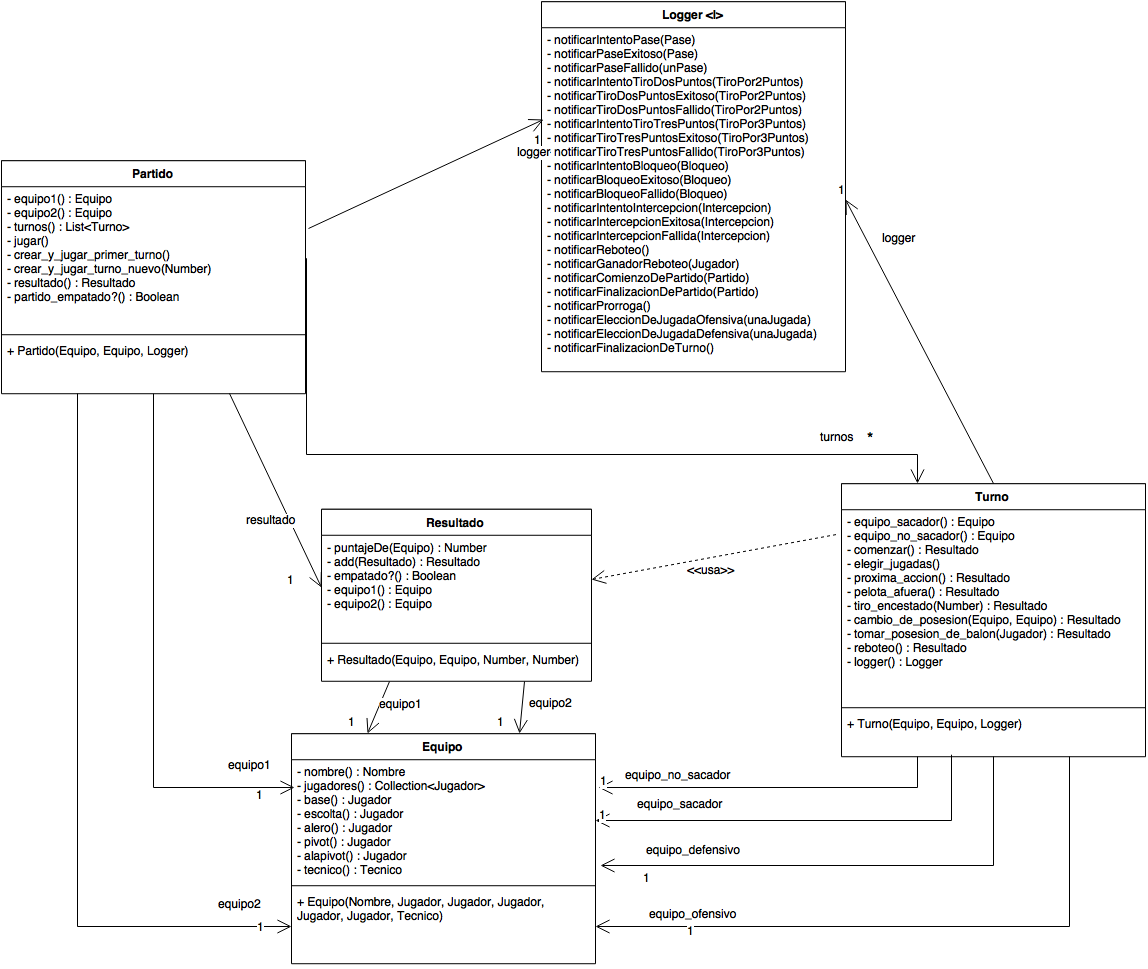
\includegraphics[scale=0.35]{imagenes/clases-partido.png}
\end{center}

En el mismo podemos observar que un Partido conoce a dos Equipos, conoce una coleccion de Turnos, conoce un Resultado que juegan el mismo y ademas conoce un Logger el cual es usado para ir dejando registro de las cosas sucedidas en el partido, lo cual ahondaremos mas en profundidad mas adelante.

De esta forma el Partido tiene la responsabilidad de ir creando los Turnos, una vez creado un turno este se desarolla o se juega y luego el Partido recibe el Resultado del Turno y actualiza su propio Resultado. Luego el Partido crea un nuevo Turno, colocando como Equipo que comienza con la pelota al que en el Turno anterior no comenzo con la Pelota. Y asi sucesivamente hasta que se hayan completado una cantidad fija de turnos, por ejemplo 40 turnos.
Una vez finalizados los 40 turnos es responsabilidad del Partido comprobar si el Resultado esta empatado o si hay un ganador, en caso de haber un ganador se da por finalizado el Partido y devuelve a su llamador el Resultado.
Pero, en caso de estar empatado el resultadoo, el Partido sigue creando turnos hasta llegar a otra nueva cantidad fija de turnos, por ejemplo 6, y vuelve a comprobar si hay ganador o no. Se sigue este proceso hasta llegar a un momento donde tengamos un ganador y el partido se da por finalizado.

En el siguiente Diagrama de Secuencia se muestra el proceso mediante el cual un Partido resuelve el mensaje jugar, es decir el proceso explicado mas arriba. Planteamos el escenario donde tenemos un Partido que consta de 40 posiciones y los equipos participantes son Spurs y Warriors y al finalizar estos 40 turnos el resultado no es empate.

\begin{center}
  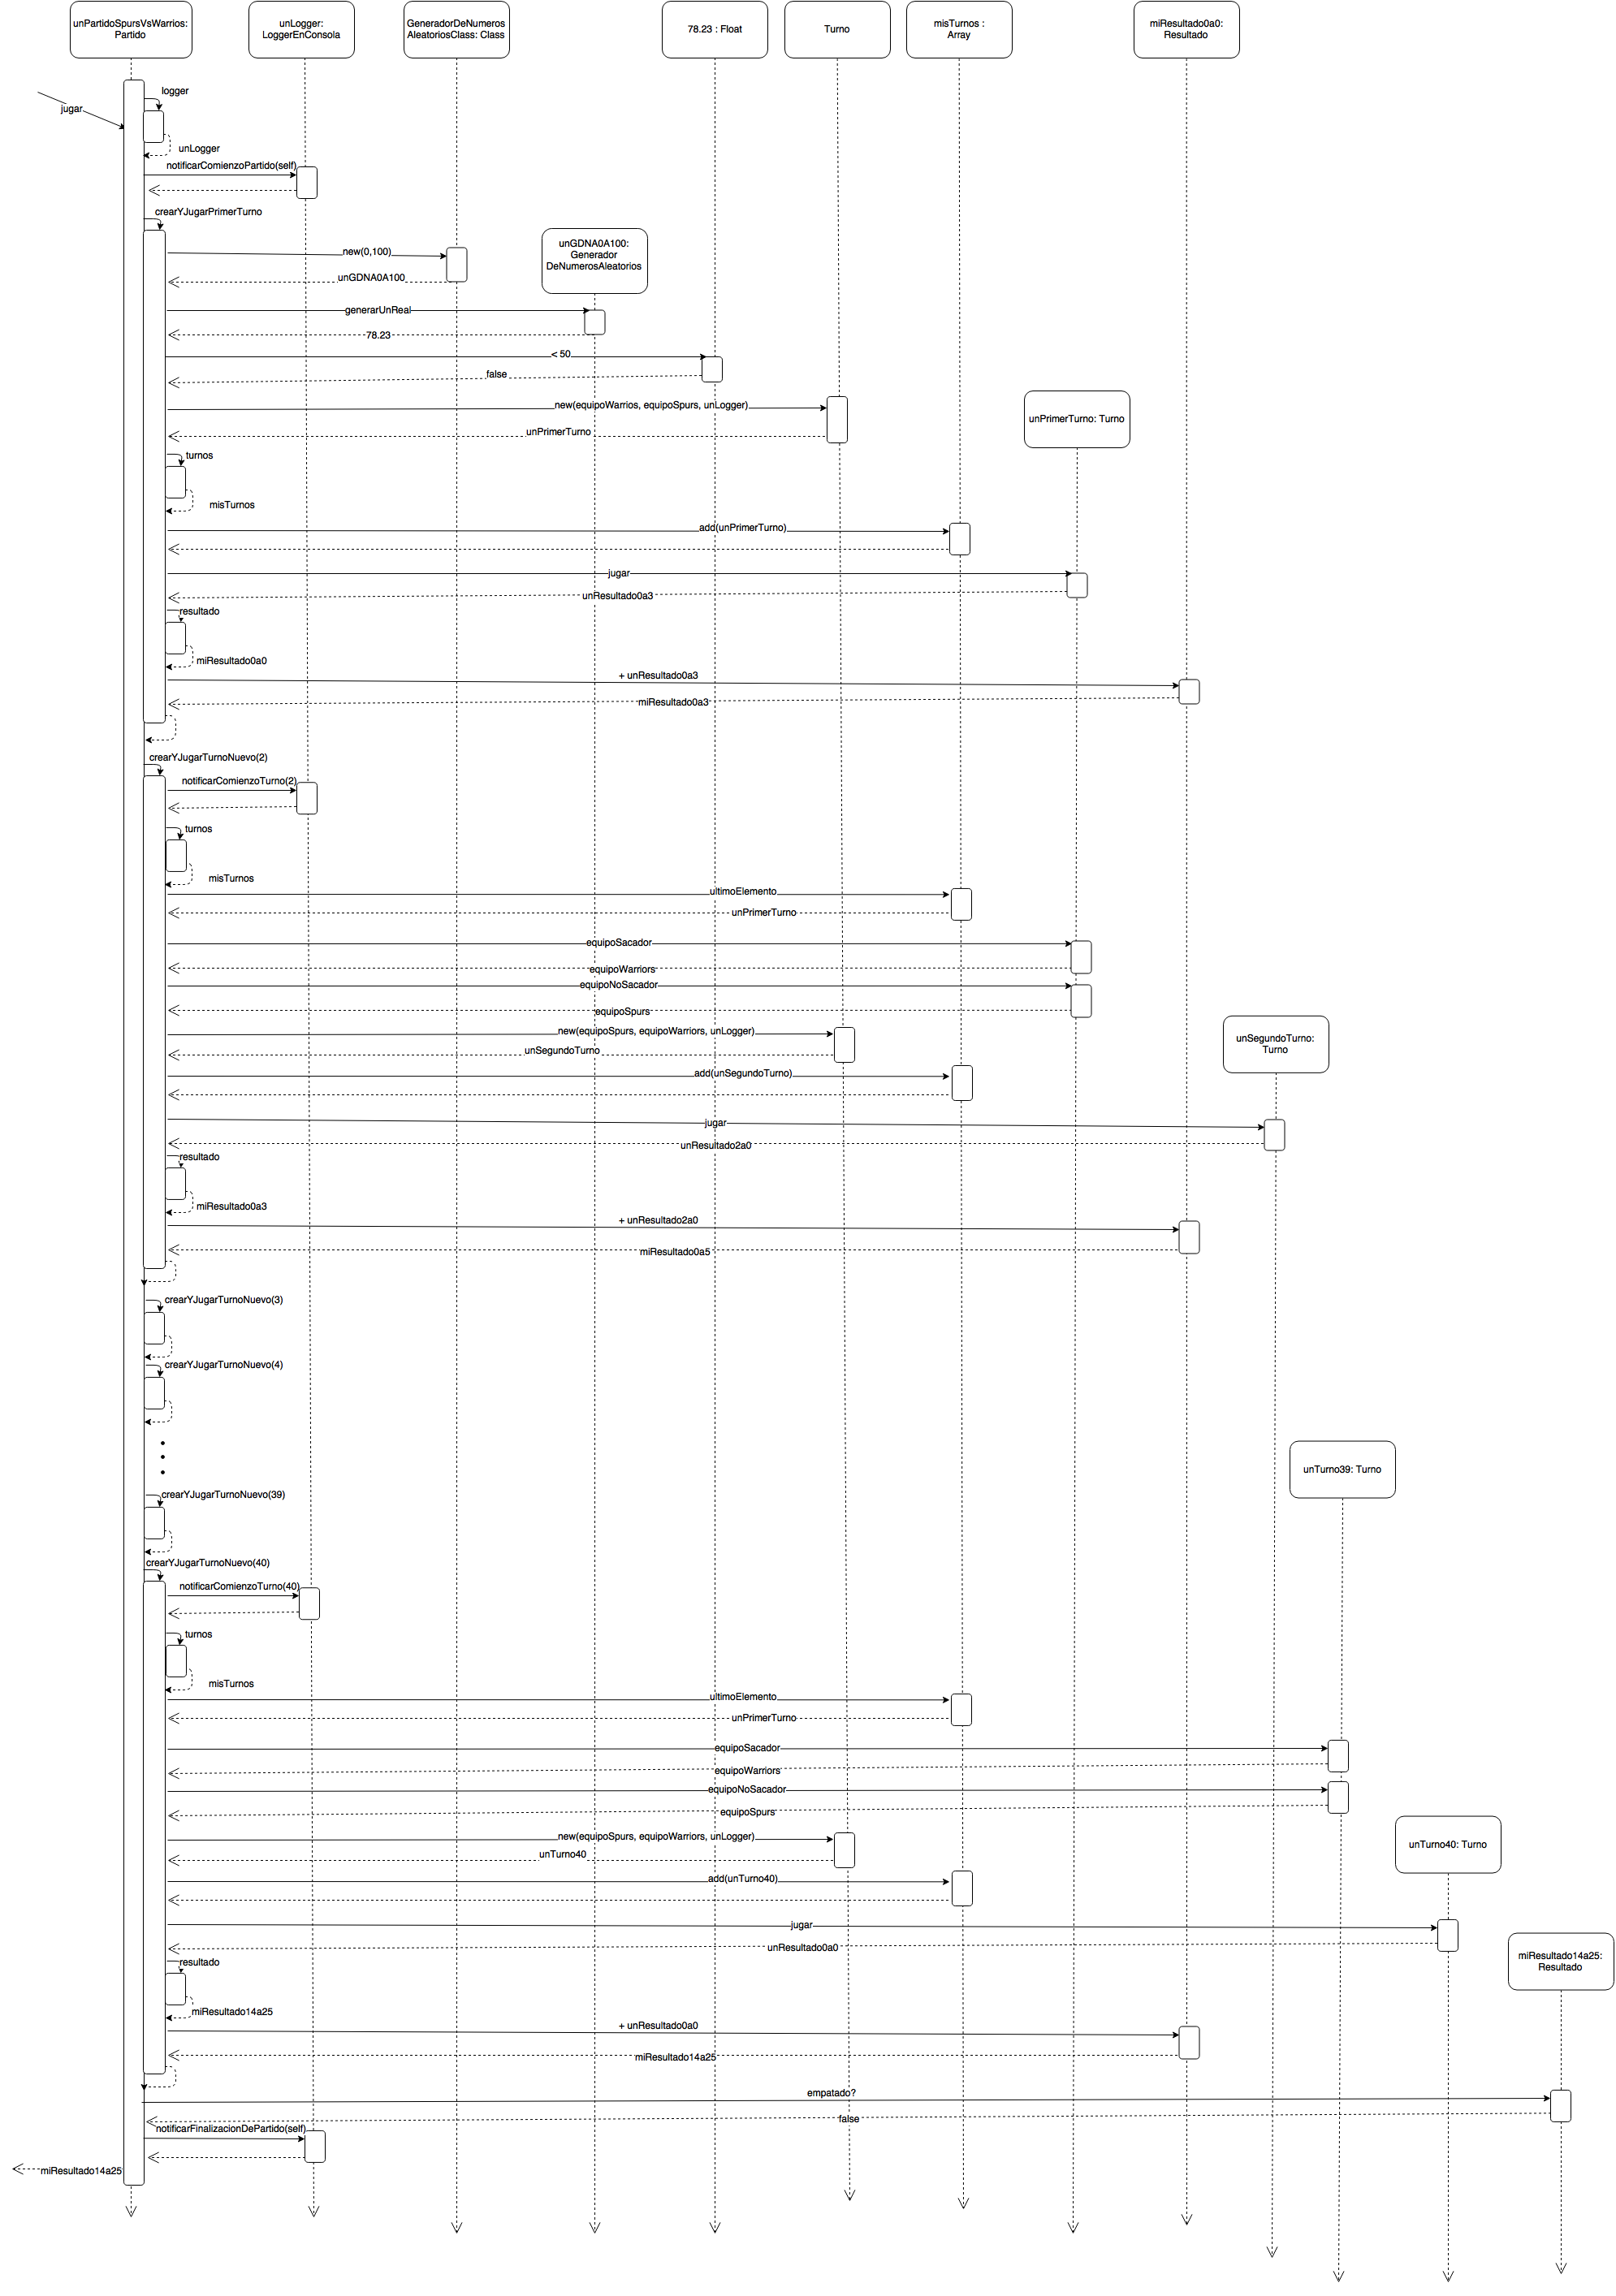
\includegraphics[scale=0.24]{imagenes/partido-jugar-secuencia.png}
\end{center}
